%% ==============
\chapter{Fundamentals}
\label{ch:Fundamentals}
%% ==============
This chapter introduces important concepts and research fundamentals that are premised throughout this work. Most of these concepts are fundamental in photorealistic rendering and thus only covered briefly, please refer to \textcite{veach1997robust} and \textcite{DBLP:conf/siggraph/Kajiya86} for a more in-depth discussion. Formulas, notations and structure of this chapter are oriented at and or cited from \textcite{lecture} and \textcite{pbrt}. Chapter~\ref{ch:Prev} will continue to cover related work that also focuses on solving lightning with many lights, but not necessarily acts as a foundation for the techniques introduced in chapter~\ref{ch:PNEE}.


\section{Rendering Equation}

In modern photorealistic rendering, the rendering equation (\ref{eq:req}) plays a central role. It describes how much radiance $L$ is emitted and reflected from a point $x$ into direction $\omega$. This serves as a physically correct representation of light transport for most observable phenomena.

\begin{align}
\label{eq:req}
L(x, \omega) =  L_e(x, \omega) + \int_{\Omega}f_r(\omega_i, x, \omega) L_i(x, \omega_i)\cos\theta_i \dif\omega_i 
\end{align}

$L_e(x, \omega)$ describes the light emission at $x$ into direction $\omega$. The integral is collecting incident light by integrating over the projected solid angle $\cos\theta_i\dif\omega_i$. $f_r(\omega_i, x, \omega)$ is called the Bidirectional Scattering Distribution Function (BSDF) and provides a factor of how much incoming light from $\omega_i$ is reflected to direction $\omega$ at point $x$. Usually, the BSDF is split up into a BRDF (Bidirectional Reflectance Distribution Function) and BTDF (Bidirectional Transmittance Distribution Function) which describe the positive hemisphere and negative hemisphere (within the material) respectively. Lastly $L_i(x, \omega_i)$ describes the incoming radiance from direction $\omega_i$. To calculate $L_i(x, \omega_i)$ a raycast is needed into direction $-\omega$. Assuming the first intersection of this ray is named $y$ $L_i(x, \omega_i)$ can be rewritten as $L(y, -\omega_i)$. Then again, $L(y, -\omega_i)$ can be calculated with the rendering equation, recursively. It is apparent that this spawns an infinite number of possible light paths and thus infinite dimensions to calculate correct light transport. To solve this only a limited number of samples can be taken to estimate the integral, this technique is discussed in section~\ref{sec:montecarlo}.

\subsection{Radiometry}


So far, we spared the conversation about the measurement units. Also, a few assumptions should be mentioned concerning the rendering equation. We assume that light ensues to the rules of geometric optics, while in fact, light has a wave-particle-dualism nature. Additionally, most computer graphic models ignore rarely visible phenomena like phosphorescence, fluorescence, polarization, relativistic effects and a few other. With this assumptions, we define that both $L$ and $L_e$ from the rendering equation are given as Radiance in $[W / (m^2sr)]$. The measurement units are assembled as follows.

\begin{align}
L = \frac{\dif E}{\cos \theta \dif\omega} = \frac{\dif^2\Phi}{\dif A\cos \theta \dif\omega} \qquad [W / (m^2 sr) ]
\end{align}


With $\cos \theta \dif\omega$ being the projected solid angle $\omega^\perp$ and $E$ being the incident light called Irrandiance, which describes the radiant flux per area.
\begin{align}
E = \frac{ \dif \Phi }{ \dif A } \qquad [W m^{-2} ]
\end{align}
Then the radiant flux $\Phi$ being the radiant energy per time given as

\begin{align}
 \Phi = \frac{\dif Q}{\dif t} \qquad [W]   
\end{align}

measured in Watt $[W = Js^{-1} ]$. And the radiant Energy $Q$ measured in Joule $[J]$. The energy $q$ of a single photon can be calculated with 

\begin{align}
 q = \frac{hc}{\lambda} \qquad [J]   
\end{align}

with $\lambda$ being the wavelength of light in nanometers, $h$ being the Planck constant $6.626~*~10^{-34}~Js$ and $c$ being the speed of light.

\subsection{Light Sources}


The radiant flux of a point light can now be set as $\Phi_g$ in $[W]$. Assuming an isotropic emission the Intensity of a point light is given as
\begin{align}
 I = \frac{\Phi_g}{4\pi} \qquad [ W sr^{-1} ] .
\end{align}

The Irradiance (incident $L$) on a sphere with radius $r$ around the point light is then given as
\begin{align}
E_r =  \frac{\Phi_g}{4\pi r^2} \qquad [ W m^{-2} ] .
\end{align}

For an area $\dif A$ the solid angle is 

\begin{align}
\dif \omega = \frac{\cos \theta \dif A}{r^2}  
\end{align}


and thus the Irradiance is

\begin{align}
E(x) = \frac{ I(\omega) \dif \omega }{ \dif A } = \frac{ \Phi_g \cos \theta }{ 4 \pi r^2}.
\end{align}

For an area light, it depends how the Radiance is modeled or given. A special case with constant radiance $L(\theta) = const$ is called a Lambertian Emitter. The intensity has to decline with $\cos\theta$, the Radiance is then given as 

\begin{align}
L(\theta) = \frac{\dif^2\Phi}{\dif\cos\theta\dif\omega}.
\end{align}



\section{Sampling}

Instead of tracing single particles in an attempt to simulate the actual physics, we choose paths that numerically represent probabilities of the physical events. \unsure{Ist das so korrekt formuliert?} As the rendering equation is continuous and infinitely recursive a numerical solution is needed to estimate it. The approximation of a definite integral with the help of random samples is called Monte Carlo Integration. Sampling describes the choice of random variables based on a given probability density to reduce the variance of these numerical methods.

\subsection{Monte Carlo Integration}
\label{sec:montecarlo}
\label{sec:MC}

To numerically approximate the definite integral over a function $f(x)$ we define $g(x) = \frac{f(x)}{p(x)}$ and instead approximate the definite integral over $g(x)p(x)$. We pick samples $x_i$ distributed according to the probability density function (section~\ref{sec:PDF}) $p(x)$ and write it as the expected value (section~\ref{sec:var}) of a random variable.

\begin{align}
E(g(x)) = \int_a^b g(x)p(x)\dif x \approx \frac{1}{N} \sum_{i=1}^{N} g(x_i) 
\end{align}

Pluging in the definition of $g(x)$ we see that we are correctly approximating the definite integral over $f(x)$ by dividing each sampled function value $f(x_i)$ by its sampling probability $p(x_i)$ and averaging them.

\begin{align}
\label{eq:mci}
\int_a^b \frac{f(x)}{p(x)}p(x)\dif x = \int_a^b f(x) \dif x \approx \frac{1}{N} \sum_{i=1}^{N} \frac{f(x_i)}{p(x_i)}
\end{align}


The rendering equation (\ref{eq:req}) then is numerically estimated as such.

\begin{align}
\label{eq:reqmc}
L(x, \omega) =  L_e(x, \omega) + \frac{2\pi}{N} \sum_{i=1}^{N} f_r(\omega_i, x, \omega) L_i(x, \omega_i)\cos\theta_i
\end{align}

Where the $2\pi$ has to be added to adjust for the fact that the integral $\int_\Omega$ over a solid angle is, in fact, a multi-dimensional integral in spherical coordinates $\int_{\phi = -\pi}^{\pi}\int_{\theta=0}^{\frac{\pi}{2}}$ and the calculation would be skewed otherwise. \unsure{Ist das so korrekt gesagt?}

\subsection{Probability Distribution Function}
\label{sec:PDF}

For a numerical solution samples (e.g. points, directions, ...) are needed, these samples can be taken for example uniformly or based on a given Probability Distribution Function (PDF). Throughout this work we refer to a PDF both in the discrete as well as in the continuous case, more strictly the discrete case is commonly referred to as Probability Mass Function (PMF) and the continuous case is referred to as Probability Density Function. Suppose that a random experiment yields random results $\omega$, we define a random Variable $X$ which maps the results to a set $\mathcal{A} \subseteq \mathbb{R}$.

\begin{align}
X: \Omega \rightarrow \mathcal{A}
\end{align}

For the discrete case, the PDF/PMF is then defined as

\begin{align}
p(x) = \Pr(X = x) = \Pr( \{\omega \in \Omega : X(\omega) = x \} ).
\end{align}

Intuitively spoken it is simply the probability of a certain outcome $x \in \mathcal{A}$ and $0$ for $x \notin \mathcal{A}$. Therefore it is apparent that the sum of probabilities has to equal to $1$.

\begin{align}
\label{eq:sum1}
\sum_{x\in\mathcal{A}}p(x) = 1
\end{align}

The cumulative distribution function (CDF) $F(x)$ is the probability that $X$ will take a value less than or equal to $x \in \mathbb{R}$.

\begin{align}
 F(x) = \Pr(X \leq x)
\end{align}

Therefore the probability that $X$ lies in the semi-closed interval $(a, b]$, where $a < b$ is  

\begin{align}
\label{eq:cdfr}
 \Pr(a \leq X < b) = F(b) - F(a).
\end{align}

For the continuous case, the probability for a specific result is always zero, for this reason, probabilities can only be given for intervals as in equation~\ref{eq:cdfr}. Hence, $p(x)$ may be viewed as the probability of $X$ sampling a value within the infinitesimal interval $[x, x + \dif x]$. The Probability Density Function $p(x)$ therefore is the slope of the CDF. The CDF can be expressed as the integral over the Probability Density Function.

\begin{align}
\label{eq:cdfc}
 F(x) = \int_{-\infty}^{x}p(t)\dif t
\end{align}

or rearranged $p(x)$ can be defined as

\begin{align}
 p(x) = \frac{\dif}{\dif x} F(x).
\end{align}

The CDF is monotonically increasing and $F(x) \in [0,1]$. The PDF is $p(t) \in [0, \infty)$ and $\int p(t)\dif t = 1$ analogous to the discrete case in equation~\ref{eq:sum1}. 

\subsection{Inverse Transform Sampling}

Having a PDF we usually now want to take random samples that are distributed according to it. Inverse Transform Sampling is one popular technique to do that. First $F(x)$ has to be constructed from the PDF like in equation~\ref{eq:cdfc}. The function then is inverted to $F^{-1}(x)$, hence the name inverse transform sampling. Now a random number $\xi$ is sampled uniformly within the range $[0, 1)$ and mapped with $F^{-1}(.)$. The resulting random variable $X$ is then distributed according to $p(x)$.

\begin{align}
 X = F^{-1}(\xi)
\end{align}

Effectively, $\xi$ constitutes the proportion of the area under $F(.)$ which is left of the sampled number $x$. Computing the inverse of the CDF analytically is often impossible, for this cases, Inverse Transform Sampling is computationally inefficient. Other methods like Rejection Sampling may apply better to these cases. In this paper we mostly work with discrete PDFs, thus inverting their CDF is always trivial by simply adding up the values.

\subsection{Variance}
\label{sec:var}
The expected value of a random variable is the sum of the possible outcomes $x_i$ multiplied with the probability of that outcome. Suppose $X$ is the random variable, for the discrete case the expected value is

\begin{align}
 E(X) = \sum_i x_i \Pr(X = x_i).
\end{align}

For the continuous case, it is 

\begin{align}
 E(X) = \int_{-\infty}^{\infty} x \cdot p(x) \dif x.
\end{align}

The law of large numbers is a theorem that describes that with many trials of an random experiment the average will be close to the expected value and with an increasing number of trials will tend to get closer. For an arbitrary $\epsilon > 0$ the following applies:

\begin{align}
 \Pr\left[ \lim_{N\rightarrow \infty} \frac{1}{N} \sum_{i=1}^N (x_i - E(X)) \leq \epsilon \right] = 1.
\end{align}

The variance is a commonly used metric to measure the deviation of a random variable $X$ from the expected value $E(X)$. It is calculated by averaging the squared deviation of each value.

\begin{align}
 \text{Var}(X) = \frac{1}{n} \sum_{i=1}^{n}(x_i - E(X))^2
\end{align}

For unbiased rendering techniques, the variance and the Mean Squared Error (MSE) usually are equal. The root of the variance is called the standard deviation $\sigma$.

\begin{align}
 \sigma(X) = \sqrt{\text{Var}(X)}
\end{align}

Again, for unbiased rendering techniques, the Root Mean Squared Error (RMSE) is usually equal to the standard deviation.

\subsection{Importance Sampling}
\label{sec:IS}

The PDF $p(x_i)$ chosen in equation~\ref{eq:mci} to generate the samples $x_i$ is determining how well which parts of the function $f(x_i)$ are sampled and thus how fast the variance $\sigma$ is decreasing with a growing number of total samples $N$. The ideal choice for the PDF is 

\begin{align}
 p(x) = \frac{1}{\int_a^b f(x) \dif x} f(x).
\end{align}

Equation~\ref{eq:ideal} shows that plugging in this $p(x)$ and rearranging it always yields the exact solution independent of $N$.

\begin{align}
 \label{eq:ideal}
 \frac{1}{N} \sum_{i=1}^{N} \frac{f(x_i)}{p(x_i)} = \frac{\int_a^b f(x) \dif x}{N} \sum_{i=1}^N \frac{f(x_i)}{f(x_i)} = \frac{\int_a^b f(x) \dif x}{N} N = \int_a^b f(x) \dif x
\end{align}

It is apparent that this ideal choice contains the function that we are trying to estimate in the first place. As such it is not usable but rather merely indicating that the closer $p(x)$ is to $f(x)$, the lower the variance will tend to be. While a uniform distribution is the standard approach and might perform mostly average, trying to estimate $p(x)$ can either improve the result a lot or do the opposite when the wrong areas are dominantly sampled, see figure~\ref{fig:importancesample}. Hence, the goal is to find good estimations of $p(x)$ as efficiently as possible.

As the Monte Carlo Integration for the rendering equation is high-dimensional the convergence is problematic. The variance for an integral $I$ is

\begin{align}
 \sigma^2 = \frac{1}{N} \int_a^b \left( \frac{f(x)}{p(x)} - I \right)^2 p(x) \dif x.
\end{align}

and for the standard deviation the following applies:

\begin{align}
 \sigma \sim \frac{1}{\sqrt{N}}.
\end{align}

This means that the number of samples has to be quadrupled to halve the error. This makes clear that at some point increasing the number of samples isn't effective anymore and importance sampling takes an important role in improving rendering quality. This is the core idea behind PNEE. We are enriching traditional NEE which chooses samples uniformly with importance sampling so that important lights are chosen more frequently. The trick is, that as long the PDF is never zero for any value no bias is introduced, as only the variance is influenced, positively or negatively. Importance sampling can be applied to many stages of the rendering process, usually where ever a random variable is involved. 


\begin{figure}
    \centering
    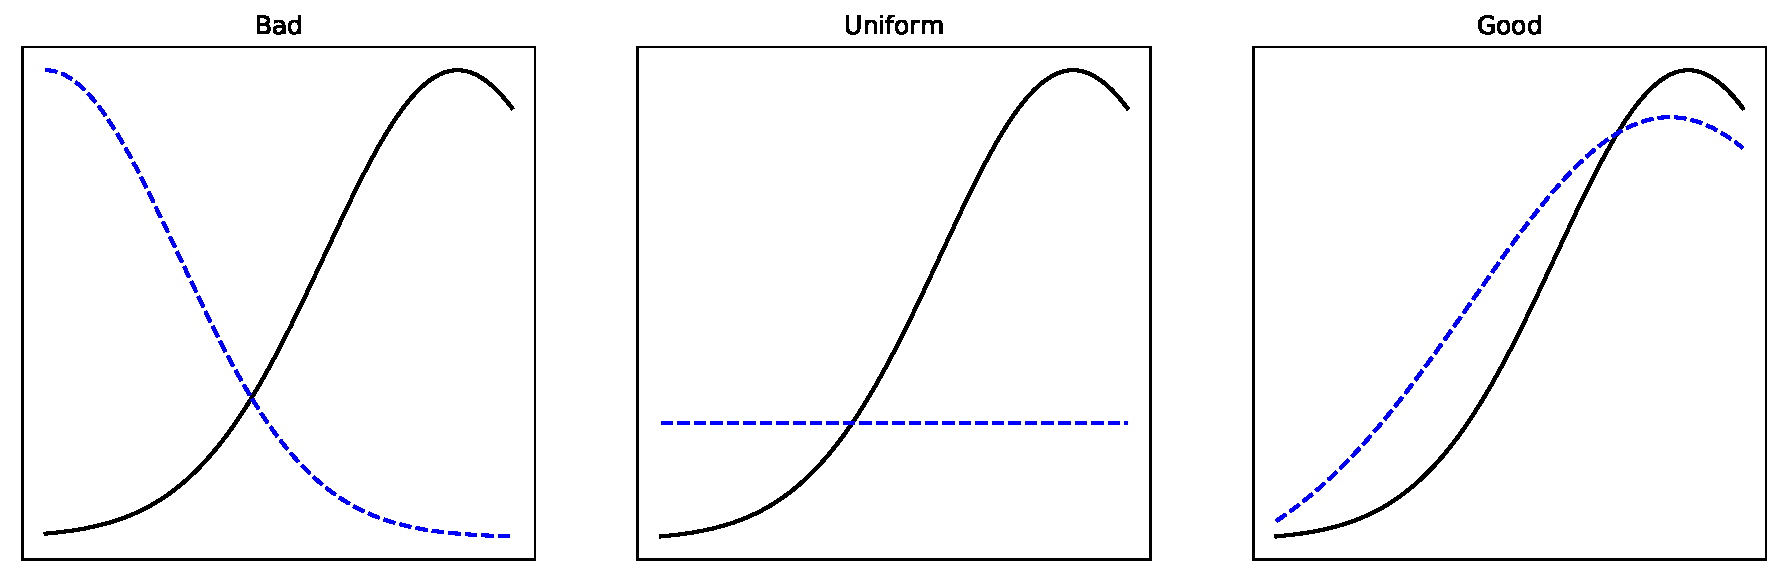
\includegraphics[width=0.8\textwidth]{figures/plots/importancesampling.pdf}
    \caption{The closer $p(x)$ estimates $f(x)$ the more useful the taken samples will be. Less samples $N$ will be needed to effectively calculate a good estimation of $f(x)$.   }
    \label{fig:importancesample}
\end{figure}

\subsection{Multiple Importance Sampling}

\section{Path Tracing}
\subsection{Next Event Estimation}
\label{sec:NEE}







%% ==============
%\section{Rendering equation}
%\subsection{Radiometry}
%\subsection{Raytracer}
%\subsection{Light Path Expressions}
%\subsection{Measurement Contribution Function}


%% ==============
%\section{Sampling}

%\subsection{Probablity Density Function}

%\subsection{Cumulative Distribution Function}

%\subsection{Inverse Transform Sampling}

%\subsection{Monte Carlo Integration}


%\subsection{Importance Sampling}
%\label{sec:IS}


%\subsection{Multiple Importance Sampling}

%% ==============
%\section{Bidirectional scattering distribution function}
% mainly only for introduction of specular vs diffuse reflections


%% ==============
%\section{Light sources}


%% ==============
%\section{Path Tracing}
%\subsection{Next Event Estimation}
%\label{sec:NEE}


%% ==============
%\section{Photon Mapping}
%\label{sec:PM}

%\subsection{Progressive Photon Mapping}

%\subsection{Stochastic Progressive Photon Mapping}



%% ==============
%\section{Instant Radiosity}

%% ==============
%\section{Datastructures}

% Teapot in a stadium ...

%\subsection{Bounding Volume Hierarchy}
%\subsection{Grid}
%\subsection{Octree}
%\subsection{k-d Tree}
%\subsection{Surface Area Heuristic}

%\section{Interpolation}
%\subsection{Scattered data}
%\subsection{Structured data}

%\label{ch:fu:trilinear}

\begin{figure}
    \centering
    
\includegraphics[width=0.5\textwidth]{figures/img-placeholder.png}
    \caption{The weights are the volume of the opposing rectangle.}
    \label{fig:bilinear}
\end{figure}
%\subsection{Global methods}


%% ==============
%\section{Machine Learning}

%\subsection{Fuzzy k-means}
%\subsection{Agglomerative Hierarchical Clustering}
%\subsection{Expectation Maximaization}
%\subsection{Transductive Support Vector Machine}